\documentclass[/home/greg/Thesis/main/main.tex]{subfiles}

%\title{Neutron star mechanics in the observers inertial frame}
%\author{}

\begin{document}
\graphicspath{{/home/greg/Neutron_star_modelling/BeamwidthCalculation/img/}}

\newcommand{\ThetaO}{\Theta_{\mathrm{obs}}}
\newcommand{\PhiO}{\Phi_{\mathrm{obs}}}
\newcommand{\sigmaB}{\sigma_{B}}
\newcommand{\Imax}{I_{\textrm{max}}}

\subsubsection{Pulse intensity}

Assuming a fixed magnitude of the magnetic dipole, the pulse intensity will
depend on the orientation of the magnetic dipole to the observer and the beam
geometry. It will be maximal when pointing directly at the observer and
presumably fall off as the angle between the two grows. To model this, we take
an observers position as $(\PhiO=0, \ThetaO)$ and then assume the beam geometry
follows Gaussian profile with a single conal emmision.
We can the express the pulse intensity for such a beam geometry as
\begin{equation}
I
(\Theta, \Phi, \ThetaO,  I_{0}, \sigmaB) 
=
I_{0} \exp\left(-\frac{\Delta d^{2}}{2\sigmaB^{2}}\right)
\label{eqn: beam intensity}
\end{equation}
where $\Theta$ and $\Phi$ are the usual beam coordinates, $I_{0}$ and $\sigmaB$
are shape parameters of the beam itself, and finally $\sigma d$ is the central
angle between the observers line of sight and the beam.
We can calulate $\Delta d$ exactly from the spherical law of cosines
\begin{equation}
\Delta\sigma = \cos^{-1}\left[\sin(\Theta)\sin(\ThetaO) +
                              \cos(\Theta)\cos(\ThetaO)\cos(|\Phi|)\right]
\label{eqn: angular sep}
\end{equation}

In figure \ref{fig: intensity variation} an illustration is given of variations
in intensity for a torque-free pulsar with some arbitary paramaters. This is
intended to demonstrate the fast rotation frequency of individual pulses, along
with the longer modulation of the precession: the parameters are artificially
selected to show both these behaviours on the same timescale.
\begin{figure}[htb]
\centering
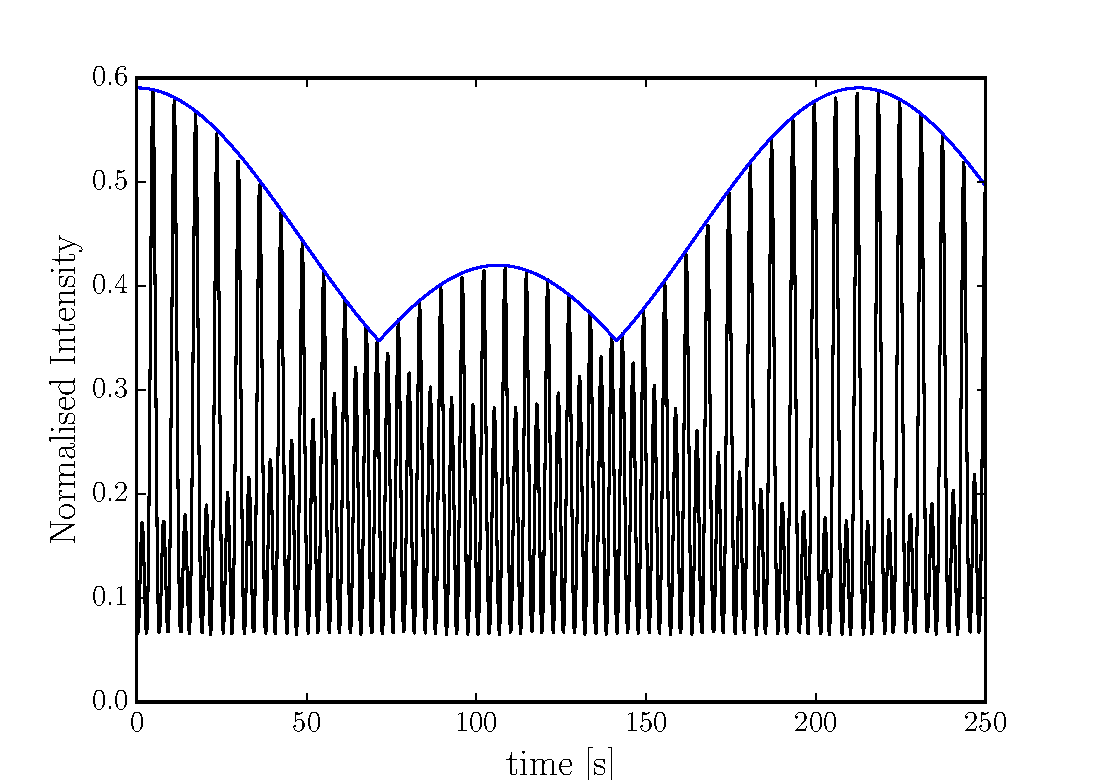
\includegraphics[width=.75\textwidth]{intensity_variation}
\caption{Amplitude variation using a 2D Gaussian emission.}
\label{fig: intensity variation}
\end{figure}•

\FloatBarrier
\subsubsection{Pulse width}
We now need to relate the pulse intensity calculated previously with the quantity
measured by pulsar astronomers: the $W_{10}$ or the width at 10\% of the peak
intensity. The subtlely here is that the peak intensity is the measured value
and not the peak of the beam (which in our model is simply  $I_0$). We will label
this measured maximum as $\Imax$ and we can see that it must occur when $\Delta d$
is at a minimum. From the functional form of Eqn.~\eqref{eqn: angular sep} we
find the minimum occurs when $\Phi=0$ in which cases we can simplify
\begin{align}
\Delta d &= \Theta - \ThetaO
\end{align}
and so
\begin{align}
\Imax = I_{0} \exp\left(-\frac{(\Theta - \ThetaO)^{2}}{2\sigmaB^{2}}\right)
\label{eqn: Imax}
\end{align}

Now let us state that $\Theta$ varies on the slow
precession timescale, while $\Phi$ varies on the rapid spin timescale. We are
looking to measure the variations with respect to the slow precession timescale.
The pulse width is measured by the time spent above some fractional amount $p/100$
of the peak measured amplitude; note the convention is to use say 10\% of the peak
value, in our notation then p=10. The condition for when the intensity is greater
than this fraction is
\begin{align}
I(\Phi, \Theta, \ThetaO, \PhiO, \sigmaB) > \Imax \frac{p}{100}.
\end{align}
We can substitute into equations~\eqref{eqn: beam intensity} and~\eqref{eqn: Imax}
and rearrange. This gives us an expression for when the inequality is satisfied:
\begin{equation}
\cos(\Phi) < \frac{\cos\left(\sqrt{\Theta - \ThetaO + 2\sigmaB^{2} \ln(\frac{p}{100})}\right) - \sin(\Theta)\sin(\ThetaO)}
                          {\cos(\Theta)\cos(\ThetaO)}
\label{eqn: 6737}
\end{equation}
Since we expect $\Theta$ to vary on a much longer timescale than $\Phi$, over 
one period in $\Phi$ we can treat $\Theta$, and hence the whole right-hand-side
as a constant. Lets consider a single rotation with the magnetic dipole
starting and ending in the antipodal point to the observers position. Then
$\Phi$ increase beween $-\pi$ and $\pi$ during this rotation. The
time during which this inequality is true, measures the beam width.

In figure \ref{fig: CosineIllustration} an illustration is given of this single
period showing the constant value on the right hand side of \eqref{eqn: 6737} and
the osciallting cosine function. When the cosine is less than this constant
this inequality is satisfied.
\begin{figure}[h!]
\centering
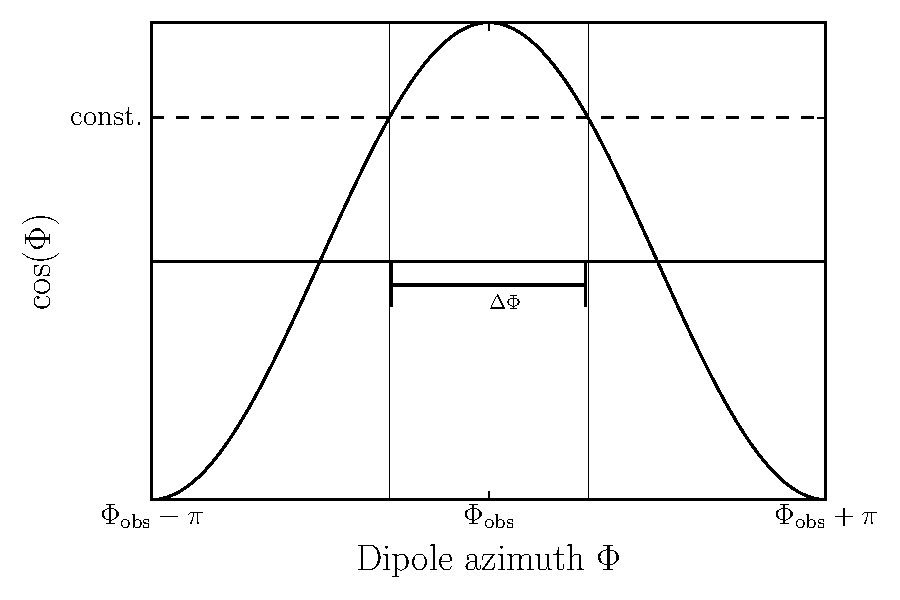
\includegraphics[width=.4\textwidth]{CosineIllustration.pdf}
\caption{Illustration of the inequality in equation \eqref{eqn: 6737} the constant
         value represents the right hand side of this equation. The
         width $\Delta\Phi$ indicates the angular period during which inequality
         is satisfied.}
\label{fig: CosineIllustration}
\end{figure}

We can calculate the beam width measured by observed by first calculating the
angular width $\Delta\Phi$ for which the inequality is not satisified:
\begin{equation}
    \Delta\Phi = 2\cos^{-1}\left(
                \frac{\cos\left(\sqrt{\Theta - \ThetaO + 2\sigmaB^{2} \ln(\frac{p}{100})}\right) - \sin(\Theta)\sin(\ThetaO)}
                          {\cos(\Theta)\cos(\ThetaO)}
                      \right)
\end{equation}
Then the angular fraction at which the inequality \emph{is} satisfied is given by
$2\pi - \Delta\Phi$. The beam width is measured in the time spent above the 
fraction $f$ of the peak measured amplitude. So we can convert our angular 
fraction above into a beam width by

We can now convert this into a pulse width 
\begin{align}
    W_p & = T \frac{2\pi - \Delta\Phi}{2\pi} \\
          & = T\left(1 -
               \frac{1}{\pi}\cos^{-1}\left(
                   \frac{\cos\left(\sqrt{\Theta - \ThetaO 
                         + 2\sigmaB^{2} \ln(\frac{100}{p})}\right)
                    - \sin(\Theta)\sin(\ThetaO)}
                          {\cos(\Theta)\cos(\ThetaO)}
                      \right)
                  \right)
\label{eqn: Wp}
\end{align}
where $T$ is the spin period which we have then written in terms of the spin
frequency and $p$ is the percentage of beam width. 
the beam width will vary with both the changes in spin-frequency, and with
$\Theta$.

%In figure \ref{fig: Pulse width modulation} we plot the beam width for some
%arbitary parameters.
%\begin{figure}[ht]
%\centering
%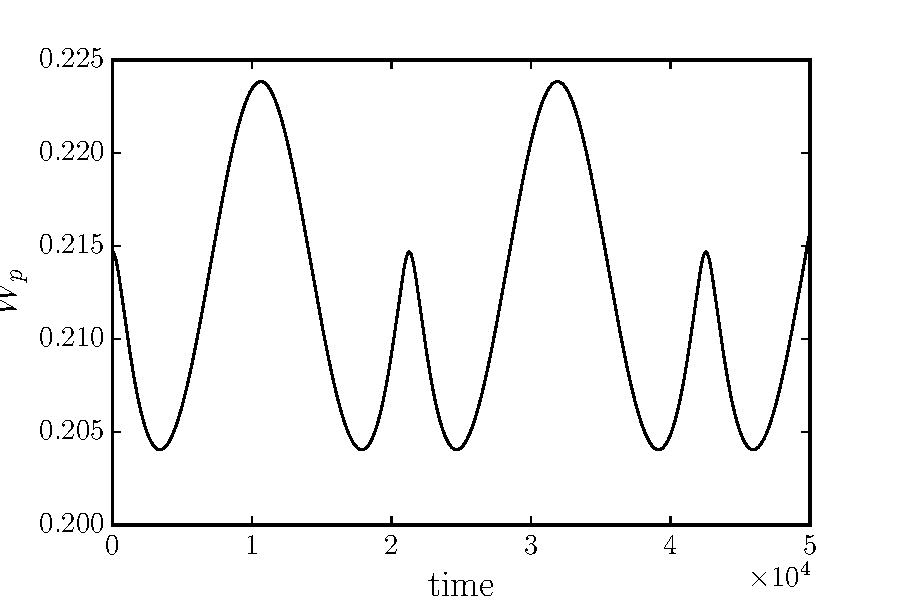
\includegraphics[width=.5\textwidth]{Pulse_width_modulation.pdf}
%\caption{}
%\label{fig: Pulse width modulation}
%\end{figure}•







%The condition for a full width half maximum at a fixed value of $\tilde{\Theta}$
%is then
%\begin{align}
%\tilde{\Phi}_{50} = \pm\sigma_{\Phi}\left(\ln(2)
%          - \frac{\tilde{\Theta}}{\sigma_{\Theta}^{2}}\right)^{1/2}
%\end{align}
%If $P$ is the period of the rapid spin motion, then the fraction $W_{50}/P$
%must be equal the fraction of the cycle spent above the full width half maximum
%which is given by $2\tilde{\Phi}_{50} / 2\pi$. Writing this in terms of the
%frequency $\dot{\Phi}$ rather than period we have
%\begin{equation}
%W_{50} = \frac{1}{\pi\dot\Phi}\sigma_{\Phi}\left(\ln(2)
%     - \frac{\tilde{\Theta}}{\sigma_{\Theta}^{2}}\right)^{1/2}
%\label{eqn: pulse width}
%\end{equation}•
%
%In figure \ref{fig: PulseWidthModulation} we plot the pulse width as a function
%of time for a canonical pulsar with $\chi=70^{\deg}$.
%\begin{figure}[ht]
%\centering
%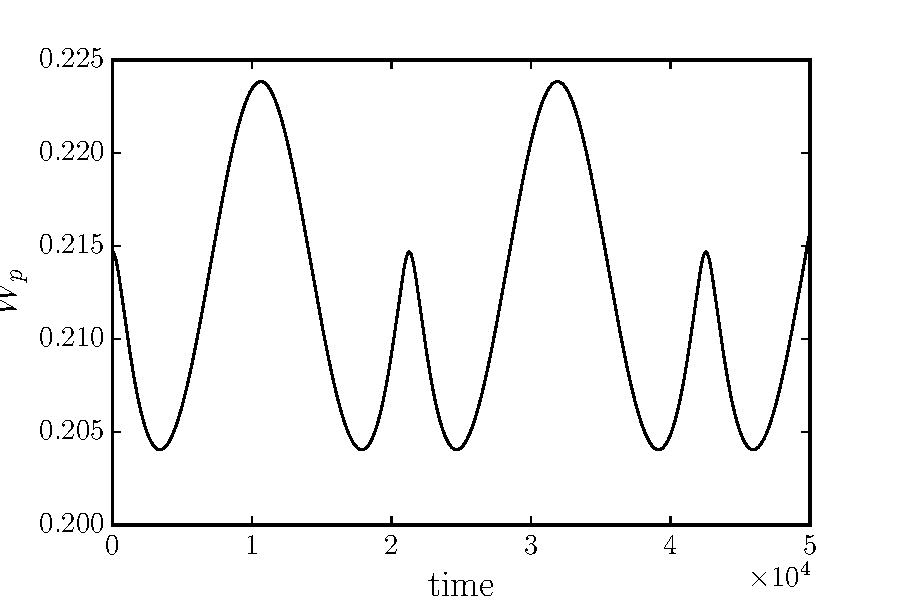
\includegraphics[width=.5\textwidth]{Pulse_width_modulation}
%\caption{Pulse width as calculated by equation \eqref{eqn: pulse width} }
%\label{fig: PulseWidthModulation}
%\end{figure}•

\FloatBarrier

\biblio
\end{document}

